\section{Introduction}
% Dennard Scaling making energy essential.  Architects address energy
% by making more complicated processors which expose resources to
% software management.  For a wide range of applications, need to meet
% performance goals with minimal energy.
Large classes of computing systems---from embedded to servers---must
deliver reliable latency while minimizing energy to prolong battery
life or lower operating costs.  To address these conflicting
requirements, hardware architects expose diverse, heterogeneous
resources with a wide array of latency and energy tradeoffs.  Software
must allocate these resources to guarantee latency requirements are
met with minimal energy.


% Difficulties of meeting latency with minimal energy. (1)
% complexity---heterogeneous resources---and (2) dynamics---adjust to
% unforeseen changes in workload and environment.
There are two primary difficulties in efficiently allocating
heterogeneous resources.  The first is \emph{complexity}: resources
interact in intricate ways, leading to non-convex optimization spaces.
The second is \emph{dynamics}: perfor\-mance requirements must be met
despite unpredictable disturbances; \eg{} changes in application
workload or operating environment.  Prior work addresses each of these
difficulties individually.

% Prior approaches addressed each of these difficulties individually.
% ML---can handle complexity.  ML advantages: can handle
% non-convexity, avoid local optima, get to true optimal solution. ML
% disadvantages: advanced techniques are expensive and no notion of
% dynamics.  Control---handles dynamics.  Control advantages: formally
% analyzable guarantees despite dynamics.  Control disadvantages:
% relies on good models---no local optima, bounded error.
Machine learning handles complex modern processors, modeling an
application's latency and power as a function of resource
configurations
\cite{reddiHPCA2013,dubach2010,Bitirgen2008,Ipek,Koala,LEO,Flicker,Ponamarev,Paragon}.
These predictions, however, are not useful if the environment changes
dynamically; \eg{} a second application enters the system.  Control
theoretic approaches dynamically adjust resource usage based on models
of the difference between measured and expected behavior
\cite{METE,Steere99,grace,Hellerstein2004a,Chen2011,POET,ControlWare,Agilos,grace2,JouleGuard}.
Control provides formal guarantees that it will meet the latency
goal in dynamic environments, but these guarantees are based on
ground-truth models relating resources and latency.  If these
models are not known or there is error between the modeled and actual
behavior, the controller will fail to deliver the required
latency.

% Want to combine learning and control to address both difficulties
% simultaneously.
%Intuitively, combining learning and control should produce predictable
%behavior in complex, dynamic systems.  There are, however, two major
%challenges to implementing the combination:
Intuitively, combining learninged models of complex hardware resources
with control-theoretic resource management should produce predictable
latency in complex, dynamic systems.  To derive the benefit of
both, however, requires addressing two major challenges:
\begin{itemize}[leftmargin=1.5em]
\item Dividing resource allocation into sub-problems that suit
  learning and control's different strengths.
\item Defining abstractions that efficiently combine sub-problem
  solutions, while maintaining control's formal guarantees.
\end{itemize}

%\PUNT{
\begin{wrapfigure}{r}{0.36\columnwidth}
%\begin{figure}[t]
\centering
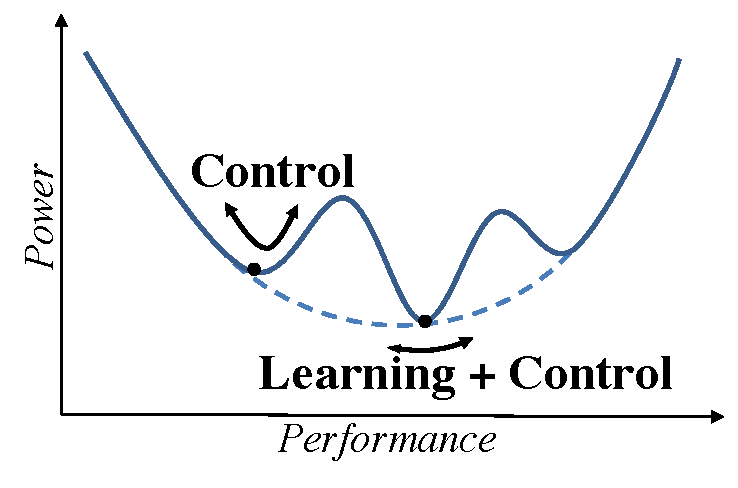
\includegraphics[width=.35\columnwidth]{figures/learning_control_doodle.pdf}
\caption{Learning smoothes the controller's domain.}
\label{fig:learning-control-doodle}
%\end{figure}
\end{wrapfigure}
%}
We address the first challenge by splitting resource allocation into
two sub-tasks.  The first is learning \emph{speedup}---instead of
absolute perf\-ormance---so that all unpredictable external
interference is viewed as a change to a \emph{baseline} latency
and the relative speedup is independent of these changes.  Learning is
well-suited to modeling speedups as a function of resource usage and
finding Pareto-optimal tradeoffs in speedup and energy.  The second
sub-task is controlling speedup dynamically based on the difference
between measured and desired latency.  Once the learner has found
Pareto-optimal tradeoffs the problem is convex and well-suited to
adaptive control solutions which guarantee the required speedup even
in dynamic environments.
%\PUNT{
\figref{fig:learning-control-doodle}
illustrates the intuition: processor complexity creates local optima,
where control solutions can get stuck; but learning finds true optimal
tradeoffs---``convexifying''---the problem, allowing control
techniques to handle dynamics while providing globally optimal energy.
%}
%Even if the measured latency
%is substantially changed due to external disturbances, the controller
%accounts for these dynamics.

We address the second challenge by defining an interface between
learning and control that maintains control's formal guarantees.  This
interface consists of two parts.  The first is a \emph{performance
  hash table} (PHT) that stores the learned model between
configurations and speedup.  The PHT allows the controller to find the
resource allocation that meets a desired speedup with minimal energy
and requires only constant time---$O(1)$---to access.  The second part
of the interface is the learned variance.  Knowing this value, the
controller can adjust itself to maintain formal guarantees even though
the speedup is modeled by a noisy learning mechanism at runtime,
rather than directly measured offline---as it would be in traditional
control design.


\emph{Thus, we propose a general methodology where an abstract control
  system is customized at runtime by a learning mechanism to meet
  latency requirements with minimal energy.} We refer to this
approach as \SYSTEM{}\footnote{\textbf{C}ontrol \textbf{A}nd
  \textbf{L}earning for \textbf{O}ptimal \textbf{R}esource
  \textbf{E}nergy \textbf{E}fficiency}.  Unlike previous work on
control systems that required numerous user-specified models and
parameters \cite{METE,Chen2011,POET,ControlWare,Agilos}, \SYSTEM{}'s
learnner tunes the control parameters automatically; \ie{} \emph{it
  requires no user-level inputs other than latency requirements}.
% Implement CALOREE.  Test against state of the art learning and
% self-tuning control systems.  We find that:
We evaluate \SYSTEM{} by implementing the learners on an x86 server
and the controller on heterogeneous ARM big.LITTLE devices.  We
compare to state-of-the-art learning (including polynomial regression
\cite{Koala,dubach2010}, collaborative filtering---\ie{} the Netflix
algorithm\cite{netflix,Paragon}---and a hierarchical Bayesian model
\cite{LEO}) and control (including proportional-integral-derivative
\cite{Hellerstein2004a} and adaptive, or self-tuning
\cite{HandbookControl}) controllers.  We set latency goals for
benchmark applications and measure both the percentage of time the
requirements are violated and the energy.  We test both
\emph{single-app}---where an application runs alone---and
\emph{multi-app} environments---where background applications enter
the system and compete for resources.  \SYSTEM{} achieves the:
\begin{itemize}[leftmargin=1em]
\item \textit{Most reliable latency:}
  \begin{itemize}[leftmargin=1em]
  \item In the \emph{single-app} case, the best prior technique misses
    10\% of deadlines on average, while \SYSTEM{} misses only 6\% on
    average. All other approaches miss 100\% of deadlines for at least
    one application, but \SYSTEM{} misses 11\% of deadlines in the
    worst case.
  \item In the \emph{multi-app} case, the best prior approach averages
    40\% deadline misses, but \SYSTEM{} misses just 20\%.
  \end{itemize}
\item \textit{Best energy savings:} We compare to an \emph{oracle}
  with a perfect model of the application, system, and future events.
  \begin{itemize}[leftmargin=1em]
  \item In the \emph{single-app} case, the best prior approach
    averages 18\% more energy consumption than the oracle, but
    \SYSTEM{} consumes only 4\% more.
  \item In the \emph{multi-app} case, the best prior approach averages
    28\% more energy than the oracle, while \SYSTEM{} consumes just
    6\% more.
  \end{itemize}
\end{itemize}

% Key contributions.
% Contributions, but I decided against bulleted llist for thsi paper
In summary, \emph{\SYSTEM{} is the first work to use learning to
  customize control systems at runtime, ensuring application
  latency---both formally and empirically---with no prior
  knowledge of the controlled application.}  Its contributions are:
\begin{itemize}[leftmargin=1em]
\item Separation of resource management into (1) \emph{learning}
  complicated resource interactions and (2) \emph{controlling}
  speedup.
\item A generalized control design for use with multiple learners.
\item A method for guaranteeing latency using learned---rather
  than measured---models.
%\item Demonstration of practical benefits using mobile/embedded
%  processors as a case study.
\end{itemize}


% Formal analysis of \SYSTEM{} demonstrates convergence
% despite noisy inputs and shows how to integrate learned variance into
% control theoretic guarantees.  We demonstrate the practical benefits
% of these contributions for mobile/embedded processors, finding
% \SYSTEM{} provides much more reliable latency and lower energy
% than learning or control solutions alone.